\documentclass[12pt]{article}
\usepackage[utf8]{inputenc}

\usepackage{amsfonts}
\usepackage{amsmath}
\usepackage{bookmark}
\usepackage[a4paper, margin=3.5cm]{geometry}
\usepackage{graphicx} % For inserting images
\usepackage{hyperref} % For hyperlinks
\usepackage{indentfirst}
\usepackage{minted} % For code-highlighting
\usepackage{parskip}

\graphicspath{ {./images/} }
\setlength{\parindent}{15pt} % Set paragraph indentation
\setlength{\parskip}{1em} % Set paragraph space (one line)
\setminted{frame=single, breaklines} % Set codeblock style

\title{Programming Practicum Report:\\Meeting \#7}
\author{\href{https://github.com/avaxar}{R. Ethan Halim}}
\date{October 21st, 2024}

\begin{document}

\maketitle

\section{Addition inside of a Function}
The entire source file is hosted on a GitHub repository \href{https://github.com/avaxar/uni-practica-1/tree/main/week_7/01_addition}{\textbf{here}}.

\subsection{Explanation}

$$\text{add}(a, b) : (\mathbb{R}, \mathbb{R}) \rightarrow \mathbb{R} = a + b$$

This is the only function that the problem necessitates. It implements addition as a function, whereby the two operands of the arithmetic operation are represented as the arguments of a function, accepting real values through the \texttt{double} data type. Similarly, it returns a real number as the result of the opaque operation. The code below is equivalent to the mathematical expression above.

\begin{minted}{cpp}
// Requirement: an addition function
double add(double a, double b) {
    return a + b;
}
\end{minted}

The main function only provides the command-line interface to interact with the function.

\begin{minted}{cpp}
int program(std::istream& cin, std::ostream& cout) {
    double a;
    cout << "a = ";
    cin >> a;

    double b;
    cout << "b = ";
    cin >> b;

    cout << "\nadd(" << a << ", " << b << ") = " << add(a, b) << '\n';
    return 0;
}
\end{minted}

% \pagebreak
\subsection{Manual Testing}
Below is the compilation and the testing of the source code.
\newline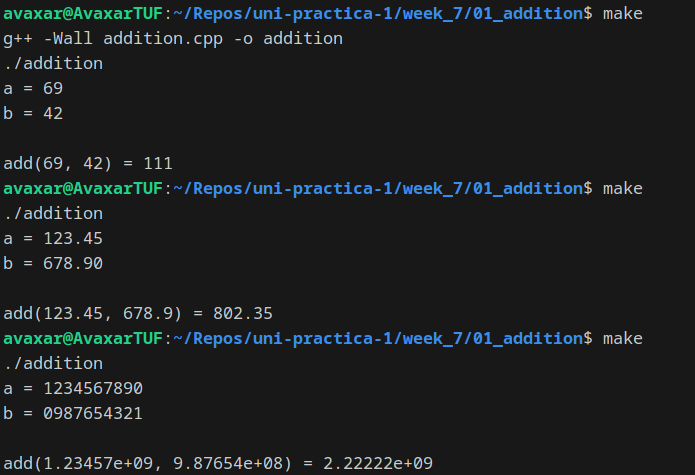
\includegraphics[width=\textwidth]{01_addition}

\pagebreak
\subsection{Test Cases}

\subsubsection{Tests}
Below is copied directly from the \texttt{tests.txt} file.
\inputminted{text}{01_addition/tests.txt}

\subsubsection{Execution}
Below are the results of the test cases. No test cases failed.
\newline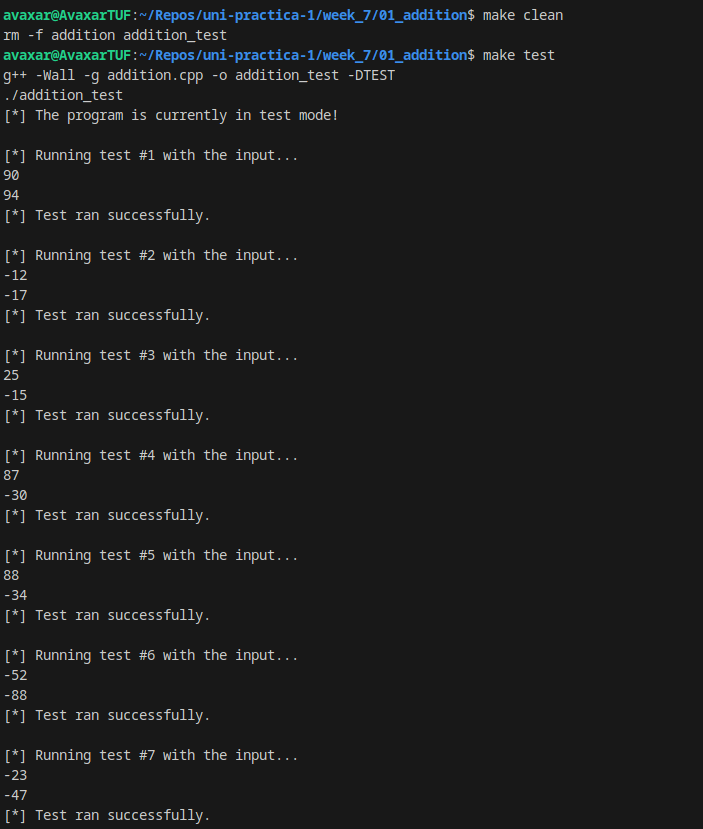
\includegraphics[width=\textwidth]{01_addition_test}

\pagebreak
\section{Recursive Function to Compute Factorials}
The entire source file is hosted on a GitHub repository \href{https://github.com/avaxar/uni-practica-1/tree/main/week_7/02_factorial}{\textbf{here}}.

\subsection{Explanation}

Mathematically, the factorial of a given natural number (an integer starting from zero) is defined as below using recursion. The end of the recursion is defined as when it hits the base case, which---in this case---is when $0!$ occurs.

$$
\text{factorial}(n) : \mathbb{N} \hat \rightarrow \mathbb{N} = n! = \begin{cases}
1 & \text{if } n = 0 \\
n \cdot (n - 1)! & \text{if } n \neq 0
\end{cases}
$$

Programmatically, it is implemented as below. In C/C++, natural numbers can be exclusively represented using unsigned integers, so the program uses the highest storing unsigned integer type---\texttt{uint64\_t}. The scenario of the base case $0!$ is checked in the initial if-statement, and an early return will be invoked following such scenario. The general case, $n \cdot (n - 1)!$, is placed following the if-statement as a return call utilizing recursion by calling its own function.

\begin{minted}{cpp}
uint64_t factorial(uint64_t n) {
    // Base case: 0! = 1
    if (n == 0) {
        return 1;
    }

    return n * factorial(n - 1);
}
\end{minted}

The main function only provides the command-line interface to interact with the function.

\begin{minted}{cpp}
int program(std::istream& cin, std::ostream& cout) {
    uint64_t n;
    cout << "n = ";
    cin >> n;

    cout << "\nfactorial(" << n << ") = " << factorial(n) << '\n';
    return 0;
}
\end{minted}

\pagebreak
\subsection{Manual Testing}
Below is the compilation and the testing of the source code.
\newline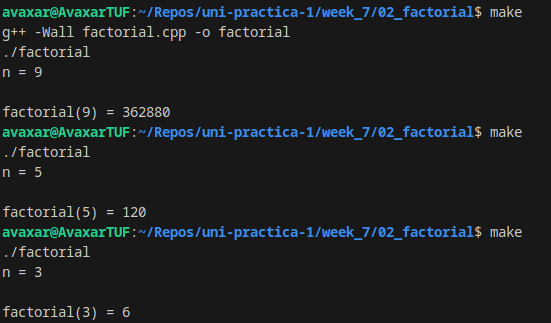
\includegraphics[width=\textwidth]{02_factorial}

% \pagebreak
\subsection{Test Cases}

\subsubsection{Tests}
Below is copied directly from the \texttt{tests.txt} file.
\inputminted{text}{02_factorial/tests.txt}

\subsubsection{Execution}
Below are the results of the test cases. No test cases failed.
\newline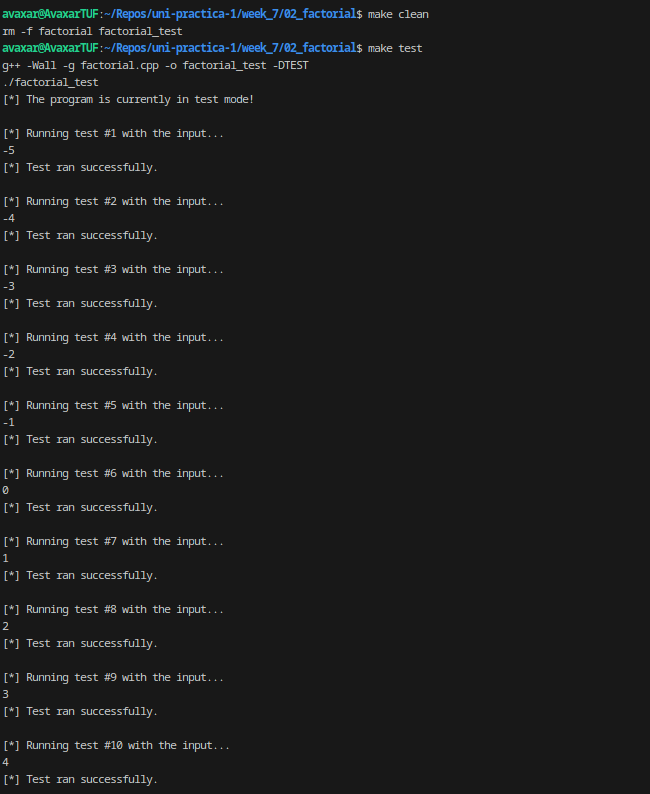
\includegraphics[width=\textwidth]{02_factorial_test}

\pagebreak
\section{Recursive Function to Compute GCDs}
The entire source file is hosted on a GitHub repository \href{https://github.com/avaxar/uni-practica-1/tree/main/week_7/03_gcd}{\textbf{here}}.

\subsection{Explanation}

Mathematically, the greatest common divisor of two given natural numbers (integers starting from zero) can be computed using the Euclidean algorithm (alternatively called ``Euclid's algorithm"), which is defined below. The algorithm utilizes recursion, wherein the final base case is when $b = 0$.

$$
\gcd(a, b) : (\mathbb{N}, \mathbb{N}) \hat \rightarrow \mathbb{N} = \begin{cases}
a & \text{if } b = 0 \\
\gcd(b, a \text{ mod } b) & \text{if } b \neq 0
\end{cases}
$$

Programmatically, it is implemented as below. In C/C++, natural numbers can be exclusively represented using unsigned integers, so the program uses the highest storing unsigned integer type---\texttt{uint64\_t}. Similar to the previous problem, the base case is checked for by an if-statement, which would perform an early return, and the general case follows it.

\begin{minted}{cpp}
// Implements the Euclidean algorithm
uint64_t gcd(uint64_t a, uint64_t b) {
    // Base case: gcd(a, 0) = a
    if (b == 0) {
        return a;
    }

    return gcd(b, a % b);
}
\end{minted}

The main function only provides the command-line interface to interact with the function.

\begin{minted}{cpp}
int program(std::istream& cin, std::ostream& cout) {
    uint64_t a;
    cout << "a = ";
    cin >> a;

    uint64_t b;
    cout << "b = ";
    cin >> b;

    cout << "\ngcd(" << a << ", " << b << ") = " << gcd(a, b) << '\n';
    return 0;
}
\end{minted}

% \pagebreak
\subsection{Manual Testing}
Below is the compilation and the testing of the source code.
\newline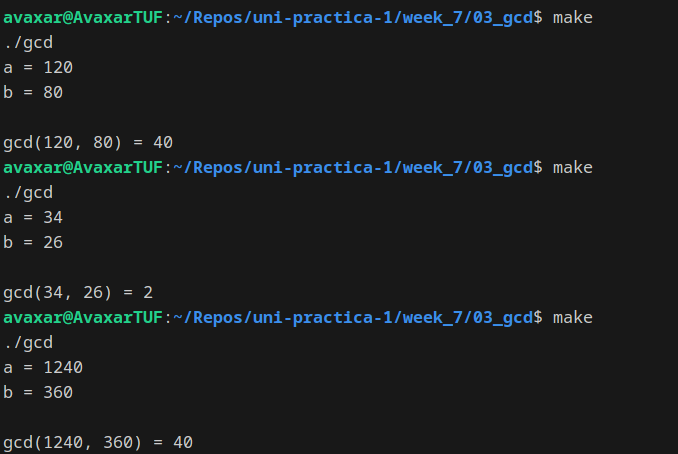
\includegraphics[width=\textwidth]{03_gcd}

% \pagebreak
\subsection{Test Cases}

\subsubsection{Tests}
Below is copied directly from the \texttt{tests.txt} file.
\inputminted{text}{03_gcd/tests.txt}

\subsubsection{Execution}
Below are the results of the test cases. No test cases failed.
\newline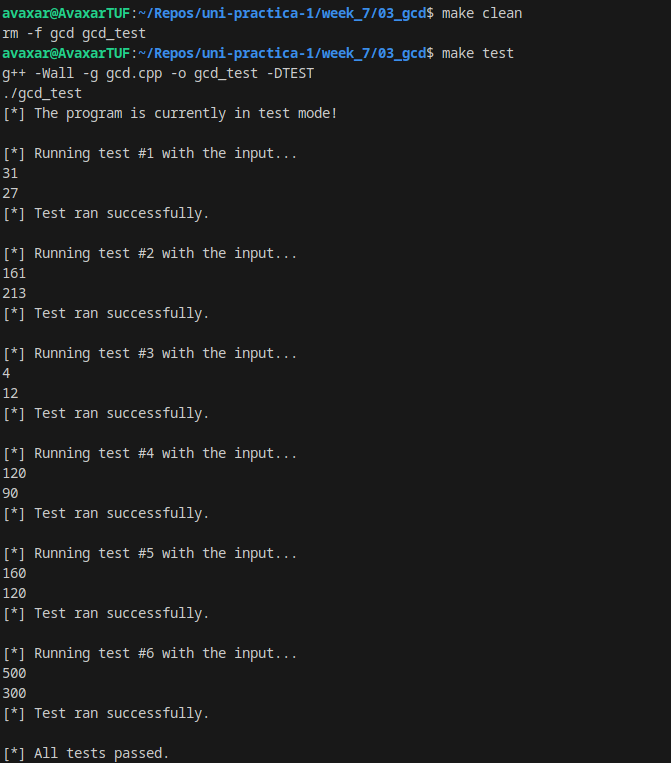
\includegraphics[width=\textwidth]{03_gcd_test}

\end{document}
